
\begin{questions}
\question{
Simple Cubic
}
\begin{solution}
Before all this we need to perform a quick calculation to know the radius of the atoms, assuming they are spherical and have a volume equal to $V_atom$,
\begin{equation}
  \begin{aligned}[b]
    V_{atom} &= \frac{4}{3}\pi r^3,\\
    \Rightarrow r_{atom} &= \left(\frac{3V_{atom}}{4\pi}\right)^{1/3}.
  \end{aligned}
  \label{radius}
\end{equation}


\begin{center}
  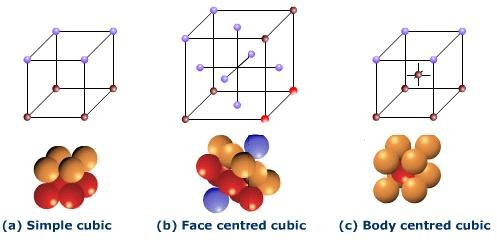
\includegraphics[width=55mm]{cells}\label{u:cells}
\end{center}

\captionof{figure}{a) SC, b) FCC and c) BC unit cells (image taken from \textit{http://chem-guide.blogspot.de/2010/04/simple-cubic-face-centered-and-body.html}).}\vspace{0.5cm}

Now that we know this we can start with the main calculations. First the atomic packing factor for the SC unit cell. For this cell we have atoms placed at the corners of a cube. They touch along the side of the cube as we can see in fig. \ref{u:cells}. Hence the length of the size of the cube is
\begin{equation*}
  a = r + 2 = 2r,
\end{equation*}
So the volume of the unit cell is
\begin{equation}
  V_{cell} = a^3 = 8r^3 =8\frac{3V_{atom}}{4\pi} =\frac{6V_{atom}}{\pi},
\end{equation}
There is just 1 atom inside the unit cell, so the atomic packing factor is going to be
\begin{equation}
  APF_{SC} = \frac{NV_{atom}}{V_{cell}} = \frac{(1)V_{atom}}{\frac{6V_{atom}}{\pi}} = \frac{\pi}{6},
\end{equation}
\end{solution}
\question{FCC}
\begin{solution}
  Now for the FCC we can see that now we have atoms at the corners and in the center of each face, so now the atoms are touching along the diagonal of the faces of the cube. So the diagonal size must be
  \begin{equation}
    c = r + 2r + r = 4r,
  \end{equation}
  but we are not interested in the diagonal, we want to know the size of the sides. We can obtain such sides with basic trigonometry, if $a$ is the side length then
  \begin{equation}
    \begin{aligned}[b]
      c^2 &= (4r)^2 = 16r^2, \\
      c^2 &= a^2 + a^2 = 2a^2,\\
      \Rightarrow 8r^2 &= a^2\\
      \Rightarrow a &= \sqrt{8}r.
    \end{aligned}
  \end{equation}
  Therefore the volume of the unit cell is
  \begin{equation}
    V_{cell} = (\sqrt{8}r)^3 = 8\sqrt{8}r^3 = 16\sqrt{2}r^3 = 16\sqrt{2}\frac{3V_{atom}}{4\pi} = \frac{12\sqrt{2}V_{atom}}{\pi} .
  \end{equation}
  The FCC cell has 4 atoms, $8*(1/8) + 6*(1/2)$, the $1/8$ comes from the atoms on the corner that are in 8 cells simultaneously and the $1/2$ comes from the atoms in the faces that are shared by two cells each. So the packing factor is
  \begin{equation}
    APF_{FCC} = \frac{4*V_{atom}}{V_{cell}} = \frac{4*V_{atom}}{\frac{12\sqrt{2}V_{atom}}{\pi}} =  \frac{\pi}{3\sqrt{2}}
  \end{equation}
\end{solution}
\end{questions}
